\documentclass[]{article}

\usepackage{fancyhdr}  % Include the package for custom headers and footers

\pagestyle{fancy}  % Change the page style to fancy to apply custom headers/footers
\fancyhf{}  % Clear all header and footer fields to start fresh
\fancyhead[R]{\thepage}  % Place the page number in the top right corner of the header
\renewcommand{\headrulewidth}{0pt}  % Remove the header rule line
\usepackage{pdflscape}
\usepackage{pdfpages}
\usepackage{graphicx}
\usepackage{subcaption}
\usepackage{colortbl}
\usepackage{booktabs}
% Beamer presentation requires \usepackage{colortbl} instead of \usepackage[table,xcdraw]{xcolor}
%opening


\newenvironment{changemargin}[2]{%
	\begin{list}{}{%
			\setlength{\topsep}{0pt}%
			\setlength{\leftmargin}{#1}%
			\setlength{\rightmargin}{#2}%
			\setlength{\listparindent}{\parindent}%
			\setlength{\itemindent}{\parindent}%
			\setlength{\parsep}{\parskip}%
		}%
		\item[]}{\end{list}}
	

\title{Neural Network Classification of Top Quark Production at the Large Hadron Collider }
\author{Raveel Tejani}



\begin{document}

\maketitle
\thispagestyle{empty}
\clearpage

\tableofcontents 
\thispagestyle{empty}
\clearpage

\listoftables
\thispagestyle{empty}
\clearpage
             
\listoffigures
\thispagestyle{empty}
\clearpage     

\section{Introduction}

At the Large Hadron Collider (LHC), where protons are collided at a staggering rate of 40 MHz across various points within the LHC ring, the ATLAS experiment plays a pivotal role as a general-purpose detector at one of these collision sites. It precisely tracks particles emitted from these collisions, an essential task for understanding fundamental physics. The integration of machine learning, specifically neural networks, is instrumental in distinguishing between different physics processes: "signals" and the more prevalent "background" events. Achieving accurate discrimination between these is crucial due to the relatively rare occurrence of signal events. The focus of this project was to explore several key objectives within the context of high-energy physics:

\begin{enumerate}
 \item Training a Classifier: Develop a neural network classifier to accurately distinguish between ttZ (the production of a pair of top quarks associated with a Z boson) and WZ (the production of a W and a Z boson) events. This distinction is critical as both ttZ and WZ can produce similar detector-level features, yet represent different underlying physics processes.
\item Feature Selection: Experiment with the addition and removal of various detector-level features to evaluate how each alteration affects the classifier's performance. This analysis helps in understanding which features are most predictive and thus critical for accurate event classification.
 \item Optimization of Neural Network: Enhance the architecture and training parameters of the neural network to maximize its performance in classifying ttZ and WZ events. This includes adjustments in network structure, learning rates, and other hyperparameters to refine the model efficacy.
 \item Feature Ranking: Determine and rank the importance of these features in the neural network to prioritize data collection and processing strategies at the detector level.

\end{enumerate}
To accomplish these goals, simulated data samples of ttZ and WZ events, produced using Monte Carlo simulations, were utilized to train the neural network. This training enables the classifier to learn the distinctive patterns of each event type. Once optimized, the classifier is then applied to actual recorded data from the LHC, using its outputs for further statistical analysis and insights. This project not only advances the accuracy and efficiency of particle identification at the ATLAS experiment but also contributes significantly to the broader field of particle physics, enhancing our understanding of particle interactions and the fundamental forces of nature.

\clearpage
\section{Methods}

Describe briefly the ML algorithms that will be used in the project

We will mainly be using a Neural Network for classification.


We are given a base model with recommended feature selection.

For the context
\begin{figure}[ht]

	\begin{subfigure}{\textwidth}
		\centering
		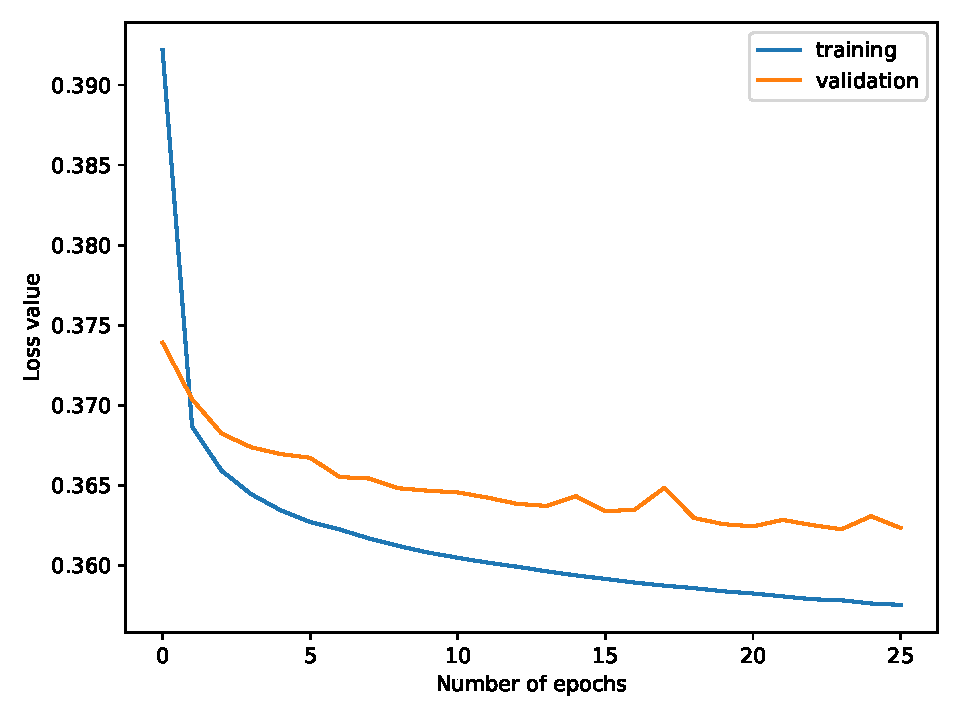
\includegraphics[height=.5\linewidth]{base_model/base_loss.pdf}
		\caption{Loss reduction as a function of epochs}
	\end{subfigure}%
	\vspace{0.2cm} % Adds space between the rows
	
	\begin{subfigure}{\textwidth}
	\centering
		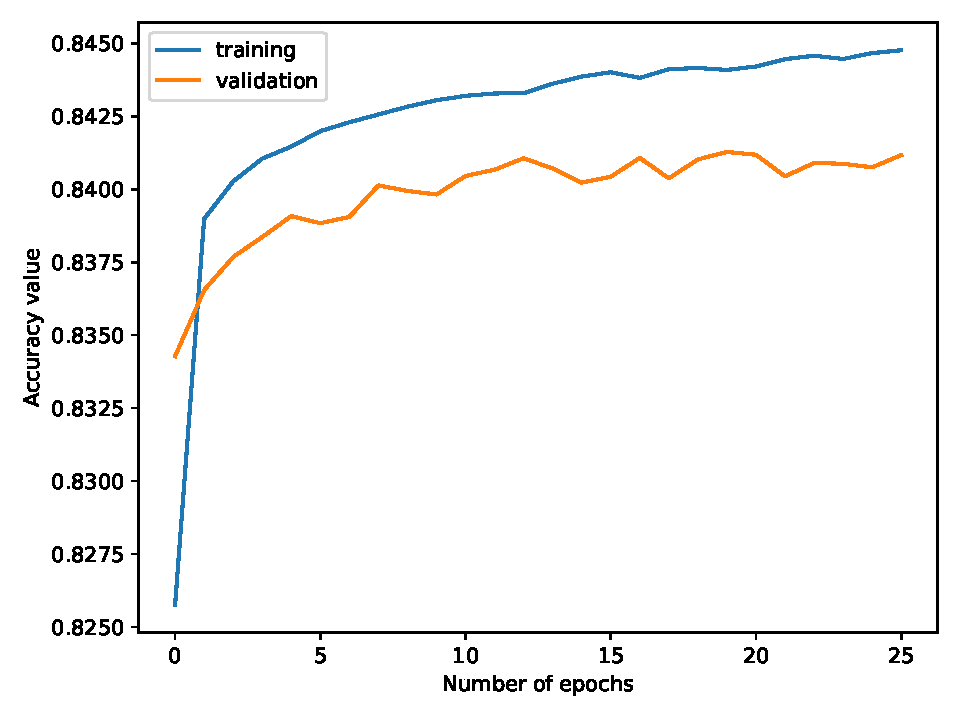
\includegraphics[height=.5\linewidth]{base_model/base_accuracy.pdf}
		\caption{Accuracy performance as a function of epochs}
	
	\end{subfigure}
	\vspace{0.2cm} % Adds space between the rows
	
	\begin{subfigure}{\textwidth}
		\centering
		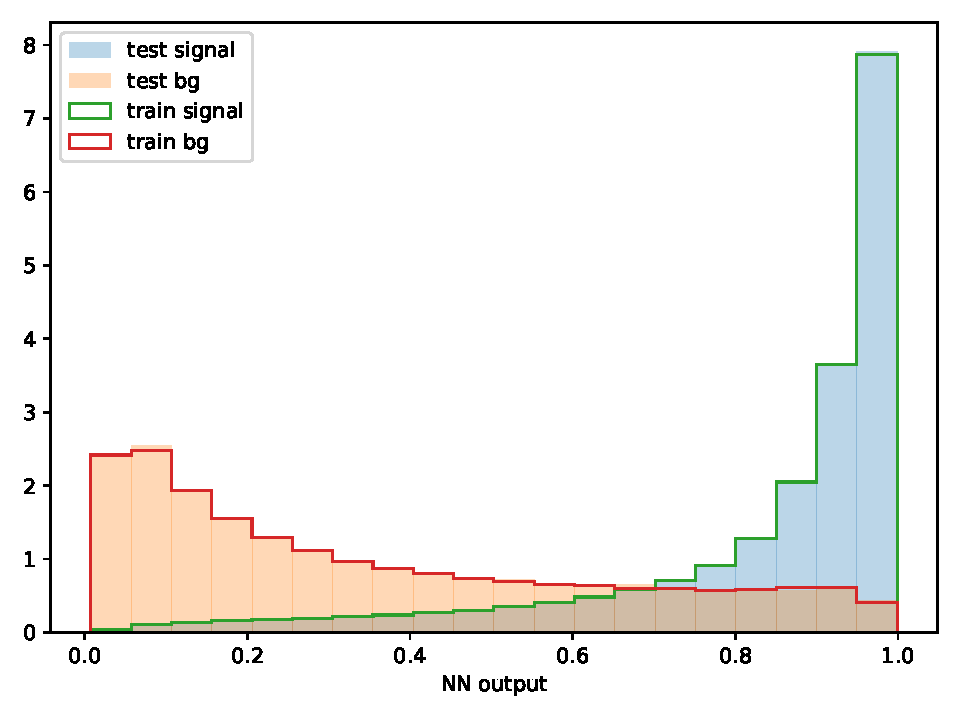
\includegraphics[height=.5\linewidth]{base_model/base_NNout.pdf}
		\caption{Probability distribution of test and train cases, based on trained Neural network}
	\end{subfigure}
	
	\caption{The base Neural Netwoek model provided  with  model.}
	\label{fig:base_model_plots}
\end{figure}


First we will start by using SRS for feature selection. Perform Base model on all features.


Then we will use gridSearch CV for model selection

We start with the base model provided with the project.

We can see the various plots generated



\clearpage
\section{Results}

Address all project questions and support your findings with appropriate graphs. Present
clearly defined figures with good layout. Make sure data interpretation is easy to infer
from figures and tables. Throughout the results, employ good practices of ML such as
cross-validation and hyperparameter optimization.



	\begin{figure}[ht]
		\centering
		\begin{subfigure}{\textwidth}
			\centering
		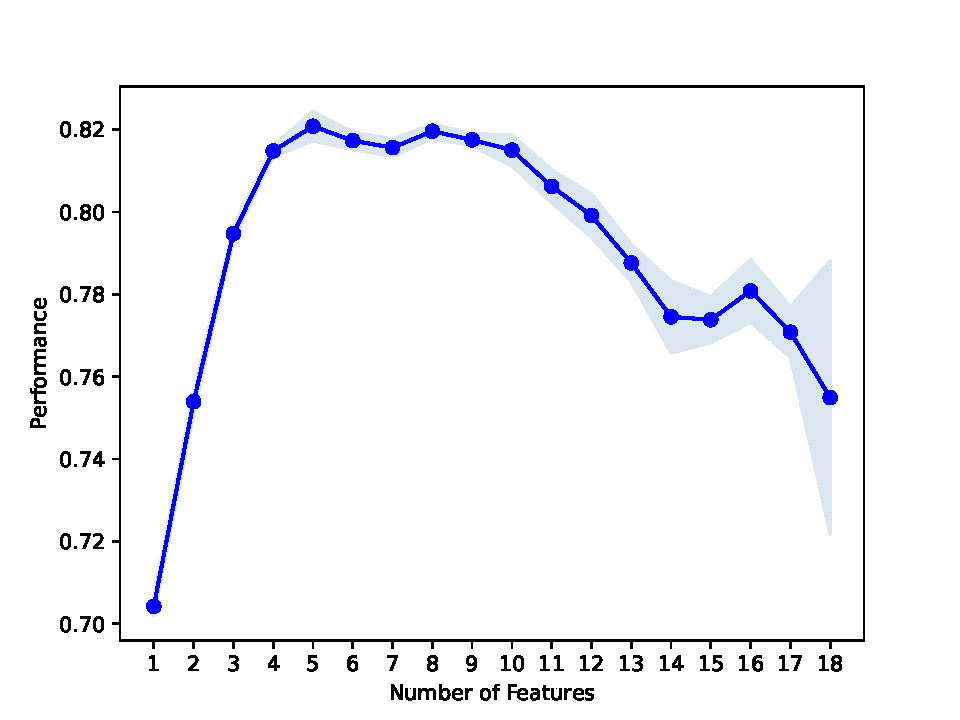
\includegraphics[width=.8\linewidth]{feature selection/feature_num_performance_10k.pdf}
		\caption{10 000 samples}
		\end{subfigure}
		\vspace{1cm} % Adds space between the images
		
		\begin{subfigure}{\textwidth}
		\centering
		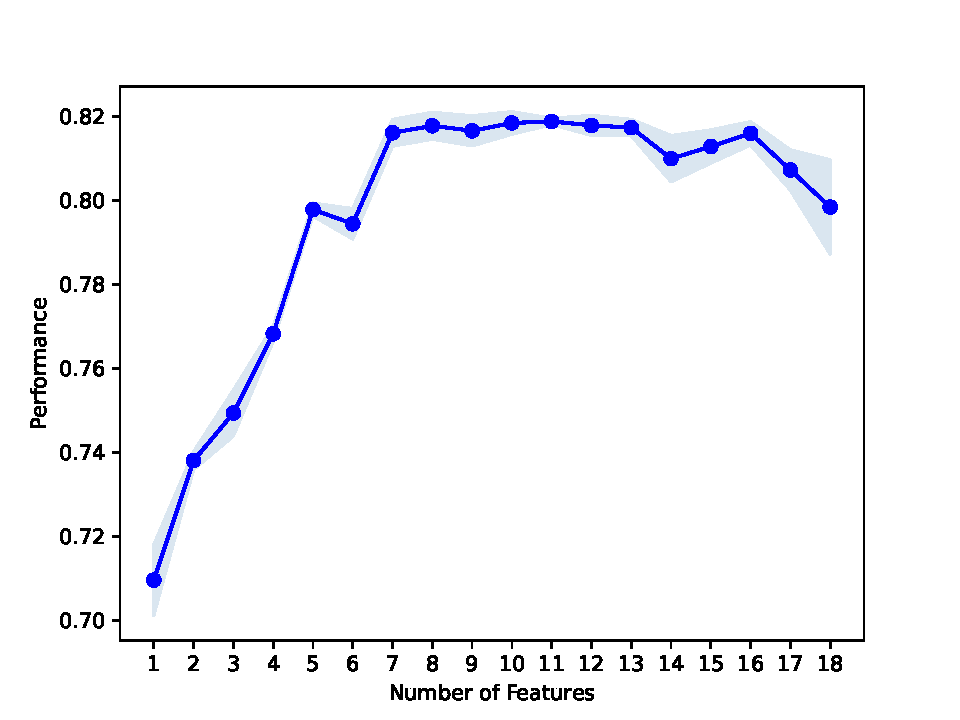
\includegraphics[width=.8\linewidth]{feature selection/feature_num_performance_30k.pdf}
		\caption{30 000 samples}
		\end{subfigure}
		\caption{The accuracy performance of Sequential Feature Selector with two subsets of the data.}
		\label{fig:SFS_results}
	\end{figure}
	
	
\begin{landscape}
\begin{table}[]
	\centering
	\resizebox{0.8\columnwidth}{!}{%
	\begin{tabular}{@{}lr@{}}
		\toprule
		Average CV Score               & Feature Names                                                                                                                                                                                                                                                                                        \\ \midrule
		70.96\%                        & ('bjet\_1\_pt',)                                                                                                                                                                                                                                                                                     \\ \addlinespace[0.5em]
		73.81\%                        & ('bjet\_1\_pt', 'n\_jets')                                                                                                                                                                                                                                                                           \\ \addlinespace[0.5em]
		74.94\%                        & ('bjet\_1\_pt', 'n\_jets', 'n\_bjets')                                                                                                                                                                                                                                                               \\ \addlinespace[0.5em]
		76.82\%                        & ('jet\_1\_twb', 'bjet\_1\_pt', 'n\_jets', 'n\_bjets')                                                                                                                                                                                                                                                \\ \addlinespace[0.5em]
		79.78\%                        & ('jet\_1\_twb', 'jet\_2\_twb', 'bjet\_1\_pt', 'n\_jets', 'n\_bjets')                                                                                                                                                                                                                                 \\ \addlinespace[0.5em]
		79.44\%                        & ('jet\_3\_pt', 'jet\_1\_twb', 'jet\_2\_twb', 'bjet\_1\_pt', 'n\_jets', 'n\_bjets')                                                                                                                                                                                                                   \\ \addlinespace[0.5em]
		\rowcolor[HTML]{32CB00} 
		81.61\%                        & ('jet\_3\_pt', 'jet\_1\_twb', 'jet\_2\_twb', 'jet\_3\_twb', 'bjet\_1\_pt',   'n\_jets', 'n\_bjets')                                                                                                                                                                                                  \\ \addlinespace[0.5em]
		81.77\%                        & \begin{tabular}[c]{@{}l@{}}('jet\_3\_pt', 'jet\_3\_eta', 'jet\_1\_twb', 'jet\_2\_twb', 'jet\_3\_twb',   'bjet\_1\_pt', 'n\_jets',\\ 'n\_bjets')\end{tabular}                                                                                                                                         \\ \addlinespace[0.5em]
		81.65\%                        & \begin{tabular}[c]{@{}l@{}}('jet\_3\_pt', 'jet\_1\_eta', 'jet\_3\_eta', 'jet\_1\_twb', 'jet\_2\_twb',   'jet\_3\_twb', 'bjet\_1\_pt',\\ 'n\_jets', 'n\_bjets')\end{tabular}                                                                                                                          \\ \addlinespace[0.5em]
		81.84\%                        & \begin{tabular}[c]{@{}l@{}}('jet\_3\_pt', 'jet\_1\_eta', 'jet\_3\_eta', 'jet\_1\_twb', 'jet\_2\_twb',   'jet\_3\_twb', 'bjet\_1\_pt',\\ 'n\_jets', 'n\_bjets', 'n\_leptons')\end{tabular}                                                                                                            \\ \addlinespace[0.5em]
		\rowcolor[HTML]{32CB00} 
		{\color[HTML]{000000} 81.88\%} & {\color[HTML]{000000} \begin{tabular}[c]{@{}l@{}}('jet\_1\_pt', 'jet\_3\_pt', 'jet\_1\_eta', 'jet\_3\_eta', 'jet\_1\_twb',   'jet\_2\_twb', 'jet\_3\_twb',\\ 'bjet\_1\_pt', 'n\_jets', 'n\_bjets', 'n\_leptons')\end{tabular}}                                                                       \\ \addlinespace[0.5em]
		81.78\%                        & \begin{tabular}[c]{@{}l@{}}('jet\_1\_pt', 'jet\_3\_pt', 'jet\_1\_eta', 'jet\_3\_eta', 'jet\_1\_twb',   'jet\_2\_twb', 'jet\_3\_twb',\\ 'bjet\_1\_pt', 'lep\_1\_pt', 'n\_jets', 'n\_bjets',   'n\_leptons')\end{tabular}                                                                              \\ \addlinespace[0.5em]
		81.73\%                        & \begin{tabular}[c]{@{}l@{}}('jet\_1\_pt', 'jet\_3\_pt', 'jet\_1\_eta', 'jet\_2\_eta', 'jet\_3\_eta',   'jet\_1\_twb', 'jet\_2\_twb',\\ 'jet\_3\_twb', 'bjet\_1\_pt', 'lep\_1\_pt', 'n\_jets',   'n\_bjets', 'n\_leptons')\end{tabular}                                                               \\ \addlinespace[0.5em]
		80.99\%                        & \begin{tabular}[c]{@{}l@{}}('jet\_1\_pt', 'jet\_3\_pt', 'jet\_1\_eta', 'jet\_2\_eta', 'jet\_3\_eta',   'jet\_1\_twb', 'jet\_2\_twb',\\ 'jet\_3\_twb', 'bjet\_1\_pt', 'lep\_1\_pt', 'n\_jets',   'n\_bjets', 'n\_leptons', 'H\_T')\end{tabular}                                                       \\ \addlinespace[0.5em] 
		81.28\%                        & \begin{tabular}[c]{@{}l@{}}('jet\_1\_pt', 'jet\_3\_pt', 'jet\_1\_eta', 'jet\_2\_eta', 'jet\_3\_eta',   'jet\_1\_twb', 'jet\_2\_twb',\\ 'jet\_3\_twb', 'bjet\_1\_pt', 'lep\_1\_pt', 'n\_jets',   'n\_bjets', 'n\_leptons', 'met\_met', 'H\_T')\end{tabular}                                           \\ \addlinespace[0.5em]
		81.59\%                        & \begin{tabular}[c]{@{}l@{}}('jet\_1\_pt', 'jet\_3\_pt', 'jet\_1\_eta', 'jet\_2\_eta', 'jet\_3\_eta',   'jet\_1\_twb', 'jet\_2\_twb',\\ 'jet\_3\_twb', 'bjet\_1\_pt', 'lep\_1\_pt', 'lep\_2\_pt',   'n\_jets', 'n\_bjets', 'n\_leptons', 'met\_met', 'H\_T')\end{tabular}                             \\ \addlinespace[0.5em]
		80.72\%                        & \begin{tabular}[c]{@{}l@{}}('jet\_1\_pt', 'jet\_3\_pt', 'jet\_1\_eta', 'jet\_2\_eta', 'jet\_3\_eta',   'jet\_1\_twb', 'jet\_2\_twb',\\ 'jet\_3\_twb', 'bjet\_1\_pt', 'lep\_1\_pt', 'lep\_2\_pt',   'lep\_3\_pt', 'n\_jets', 'n\_bjets', 'n\_leptons', 'met\_met', 'H\_T')\end{tabular}               \\ \addlinespace[0.5em]
		79.84\%                        & \begin{tabular}[c]{@{}l@{}}('jet\_1\_pt', 'jet\_2\_pt', 'jet\_3\_pt', 'jet\_1\_eta', 'jet\_2\_eta',   'jet\_3\_eta', 'jet\_1\_twb', 'jet\_2\_twb',\\ 'jet\_3\_twb', 'bjet\_1\_pt', 'lep\_1\_pt',   'lep\_2\_pt', 'lep\_3\_pt', 'n\_jets', 'n\_bjets', 'n\_leptons', 'met\_met', 'H\_T')\end{tabular} \\ \bottomrule
	\end{tabular}
	}
	\caption{Results of the Secquential Feature Selector. We can gather Feature Importances from these tables. The ones highlighed in green is what we use to continue our analysis}
	\label{table:SFS_results}
\end{table}

\end{landscape}



\begin{figure}[ht]
	\centering
	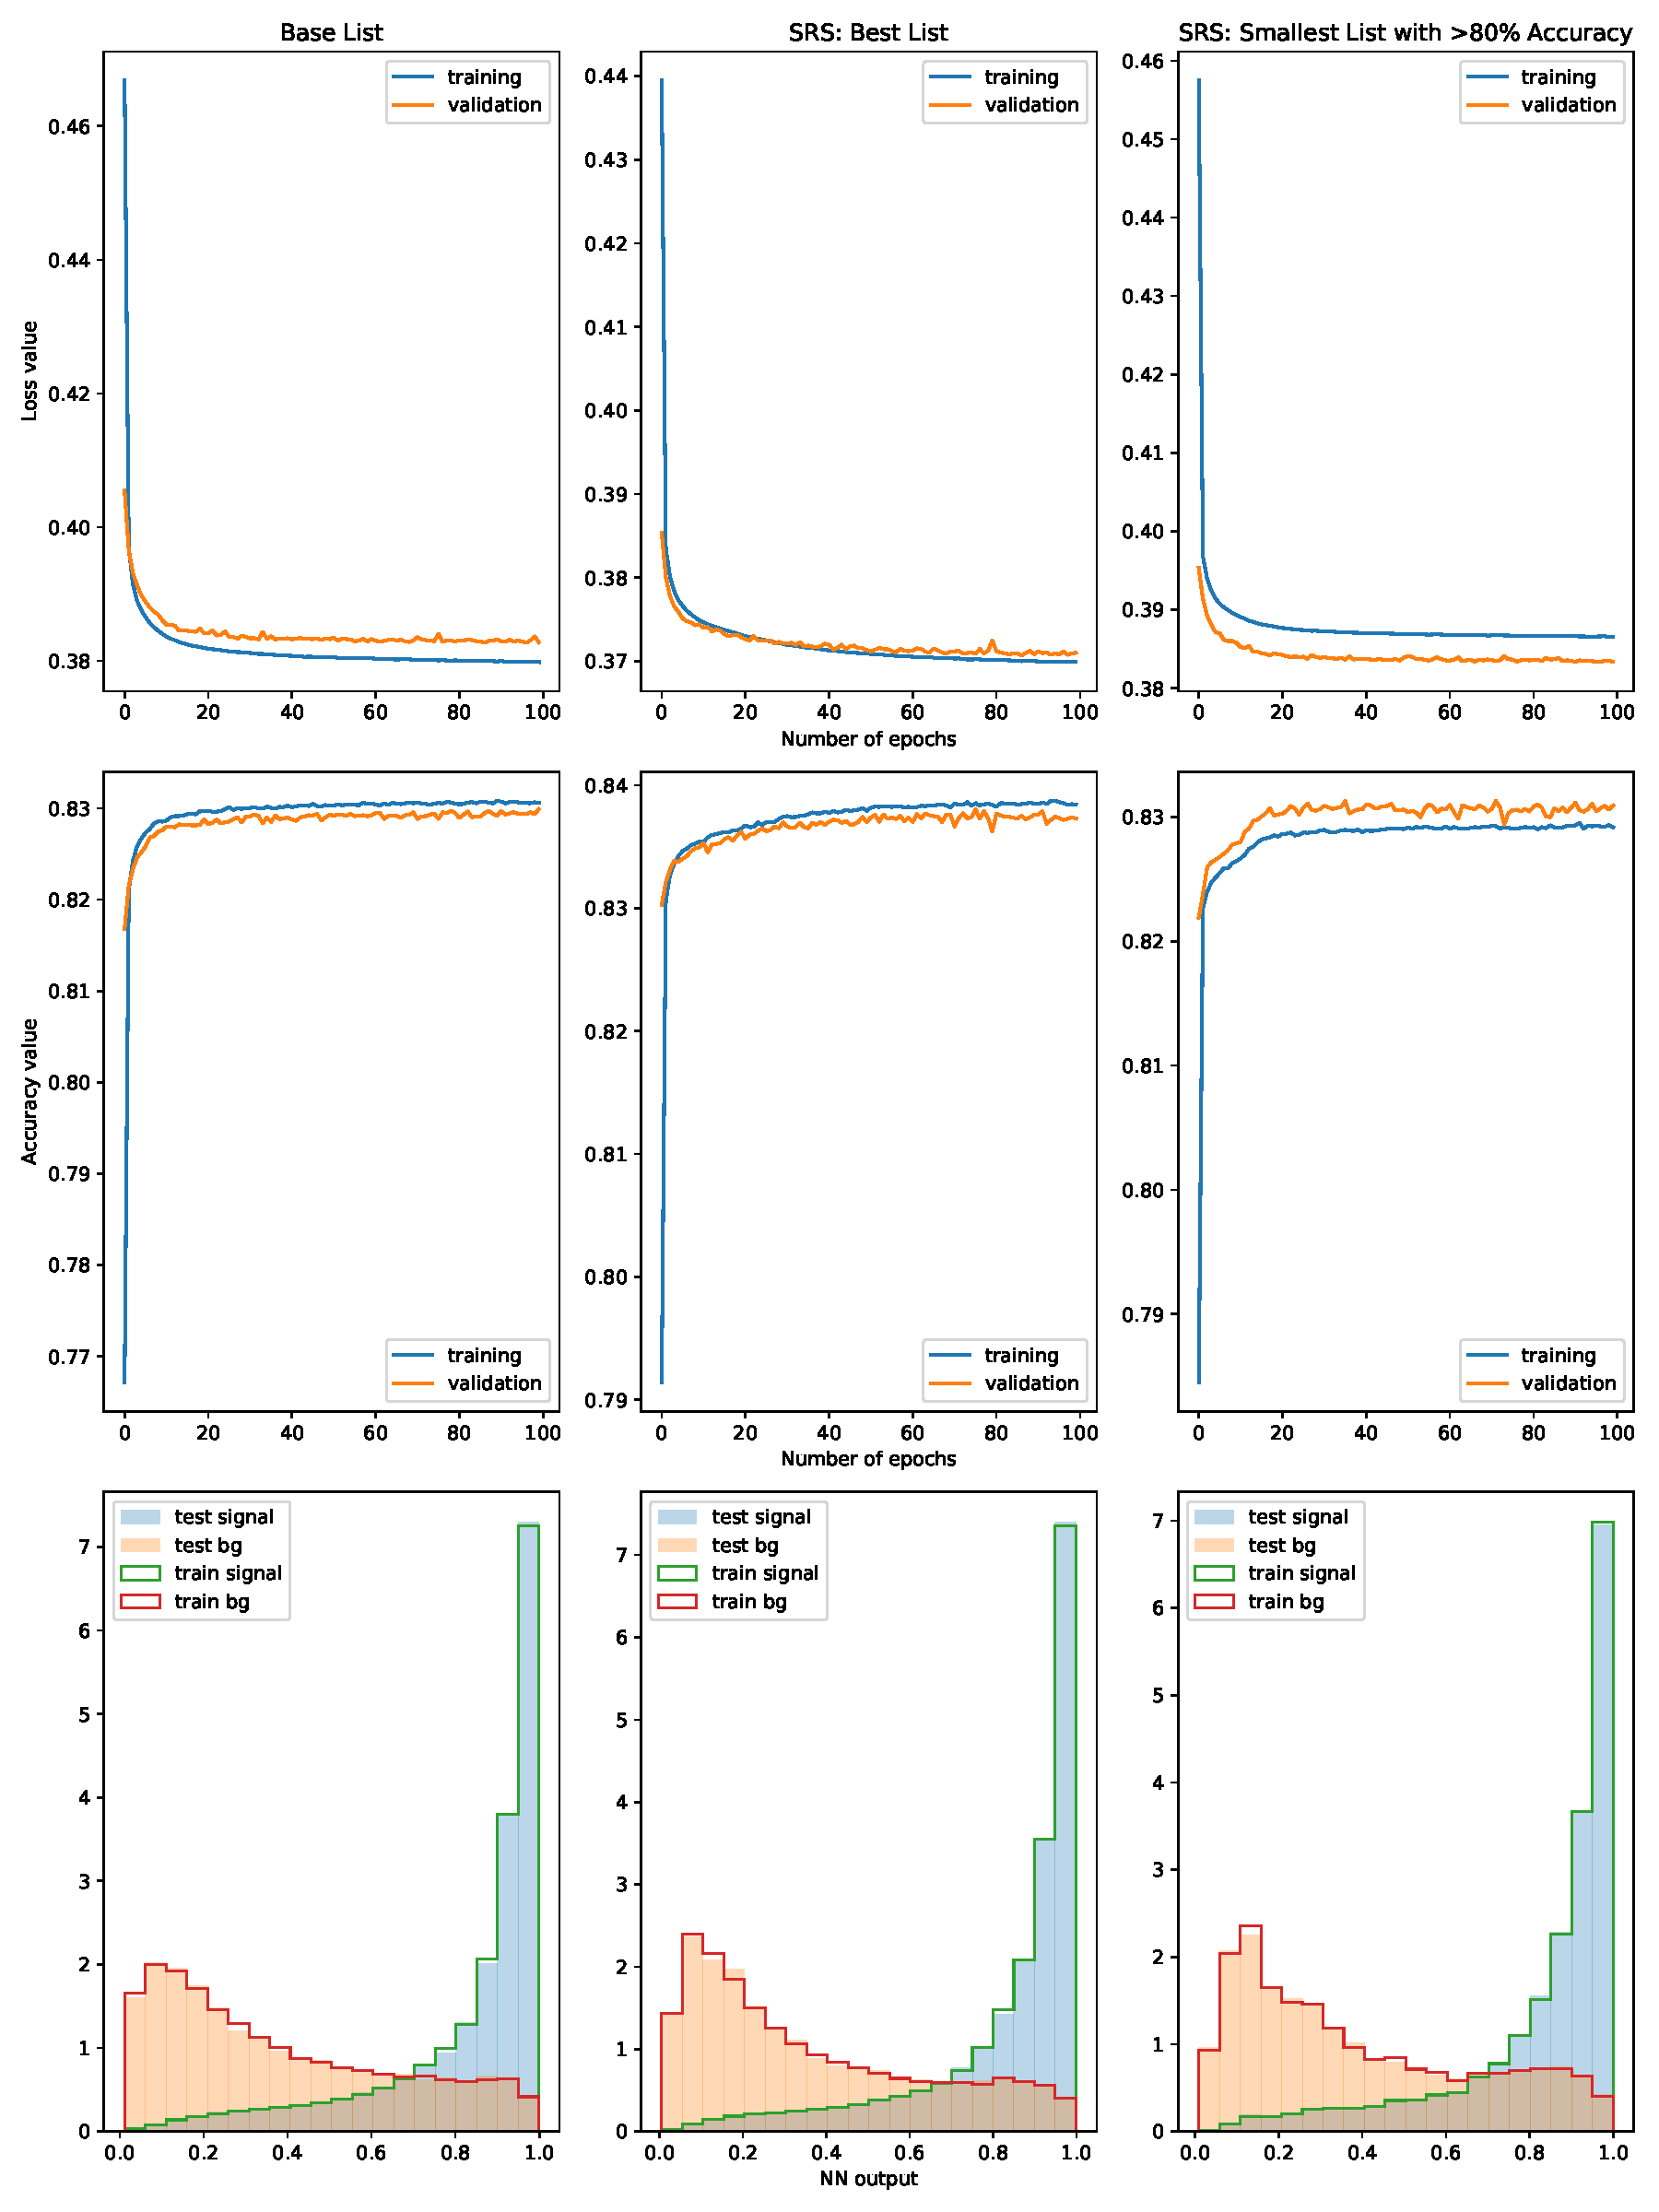
\includegraphics[width=\linewidth]{feature_comparison/feat-comparison.pdf}
	\caption{Performance plots of all 3 feature lists based on the base model provided}
	\label{fig:base_models}
\end{figure}


Model Selection:

\begin{table}[]
	\centering
	\begin{tabular}{@{}lrrr@{}}
		\toprule
		Parameter            & Trial 1 & Trial 2 & Trial 3 \\ \midrule
		Nodes: Dense Layer 1 & 25      & 50      & 100     \\
		Nodes: Dense Layer 2 & 12      & 25      & 50      \\
		Nodes: Dense Layer 3 & 5       & 10      & 15      \\
		Batch Size           & 100     & 150     & 300     \\
		Adam Learning Rate   & 0.002   & 0.0002  & 0.00002 \\
		Best Score           & 82.96\% & 83.39\% & 82.7\%\\
		\bottomrule   
	\end{tabular}
		\caption{Parameters we will swift through in gridsearchCV.} 
	\label{table:gridsearchCV_params}
\end{table}




\begin{table}[h!]
	\centering
	\begin{tabular}{@{}lrrr@{}}
		\toprule
		Parameters           & Base List & SRS: Best List & SRS: Best Small List \\ \midrule

		Nodes: Dense Layer 1 & 50        & 25             & 50                                                  \\
		Nodes: Dense Layer 2 & 12        & 25             & 50                                                  \\
		Nodes: Dense Layer 3 & 10        & 15             & 5                                                   \\
				Batch Size          & 300       & 100            & 150                                                 \\
		Adam Learning Rate   & 0.002     & 0.002          & 0.0002                                              \\
		Best Score           & 82.96\%   & 83.39\%        & 82.7\%  \\
		\bottomrule                                            
	\end{tabular}
	\caption{Best Parameters for the 3 Feature Lists.} 
	\label{table:best_params_gridsearchCV}
	
\end{table}




\begin{figure}[ht]
	\centering
	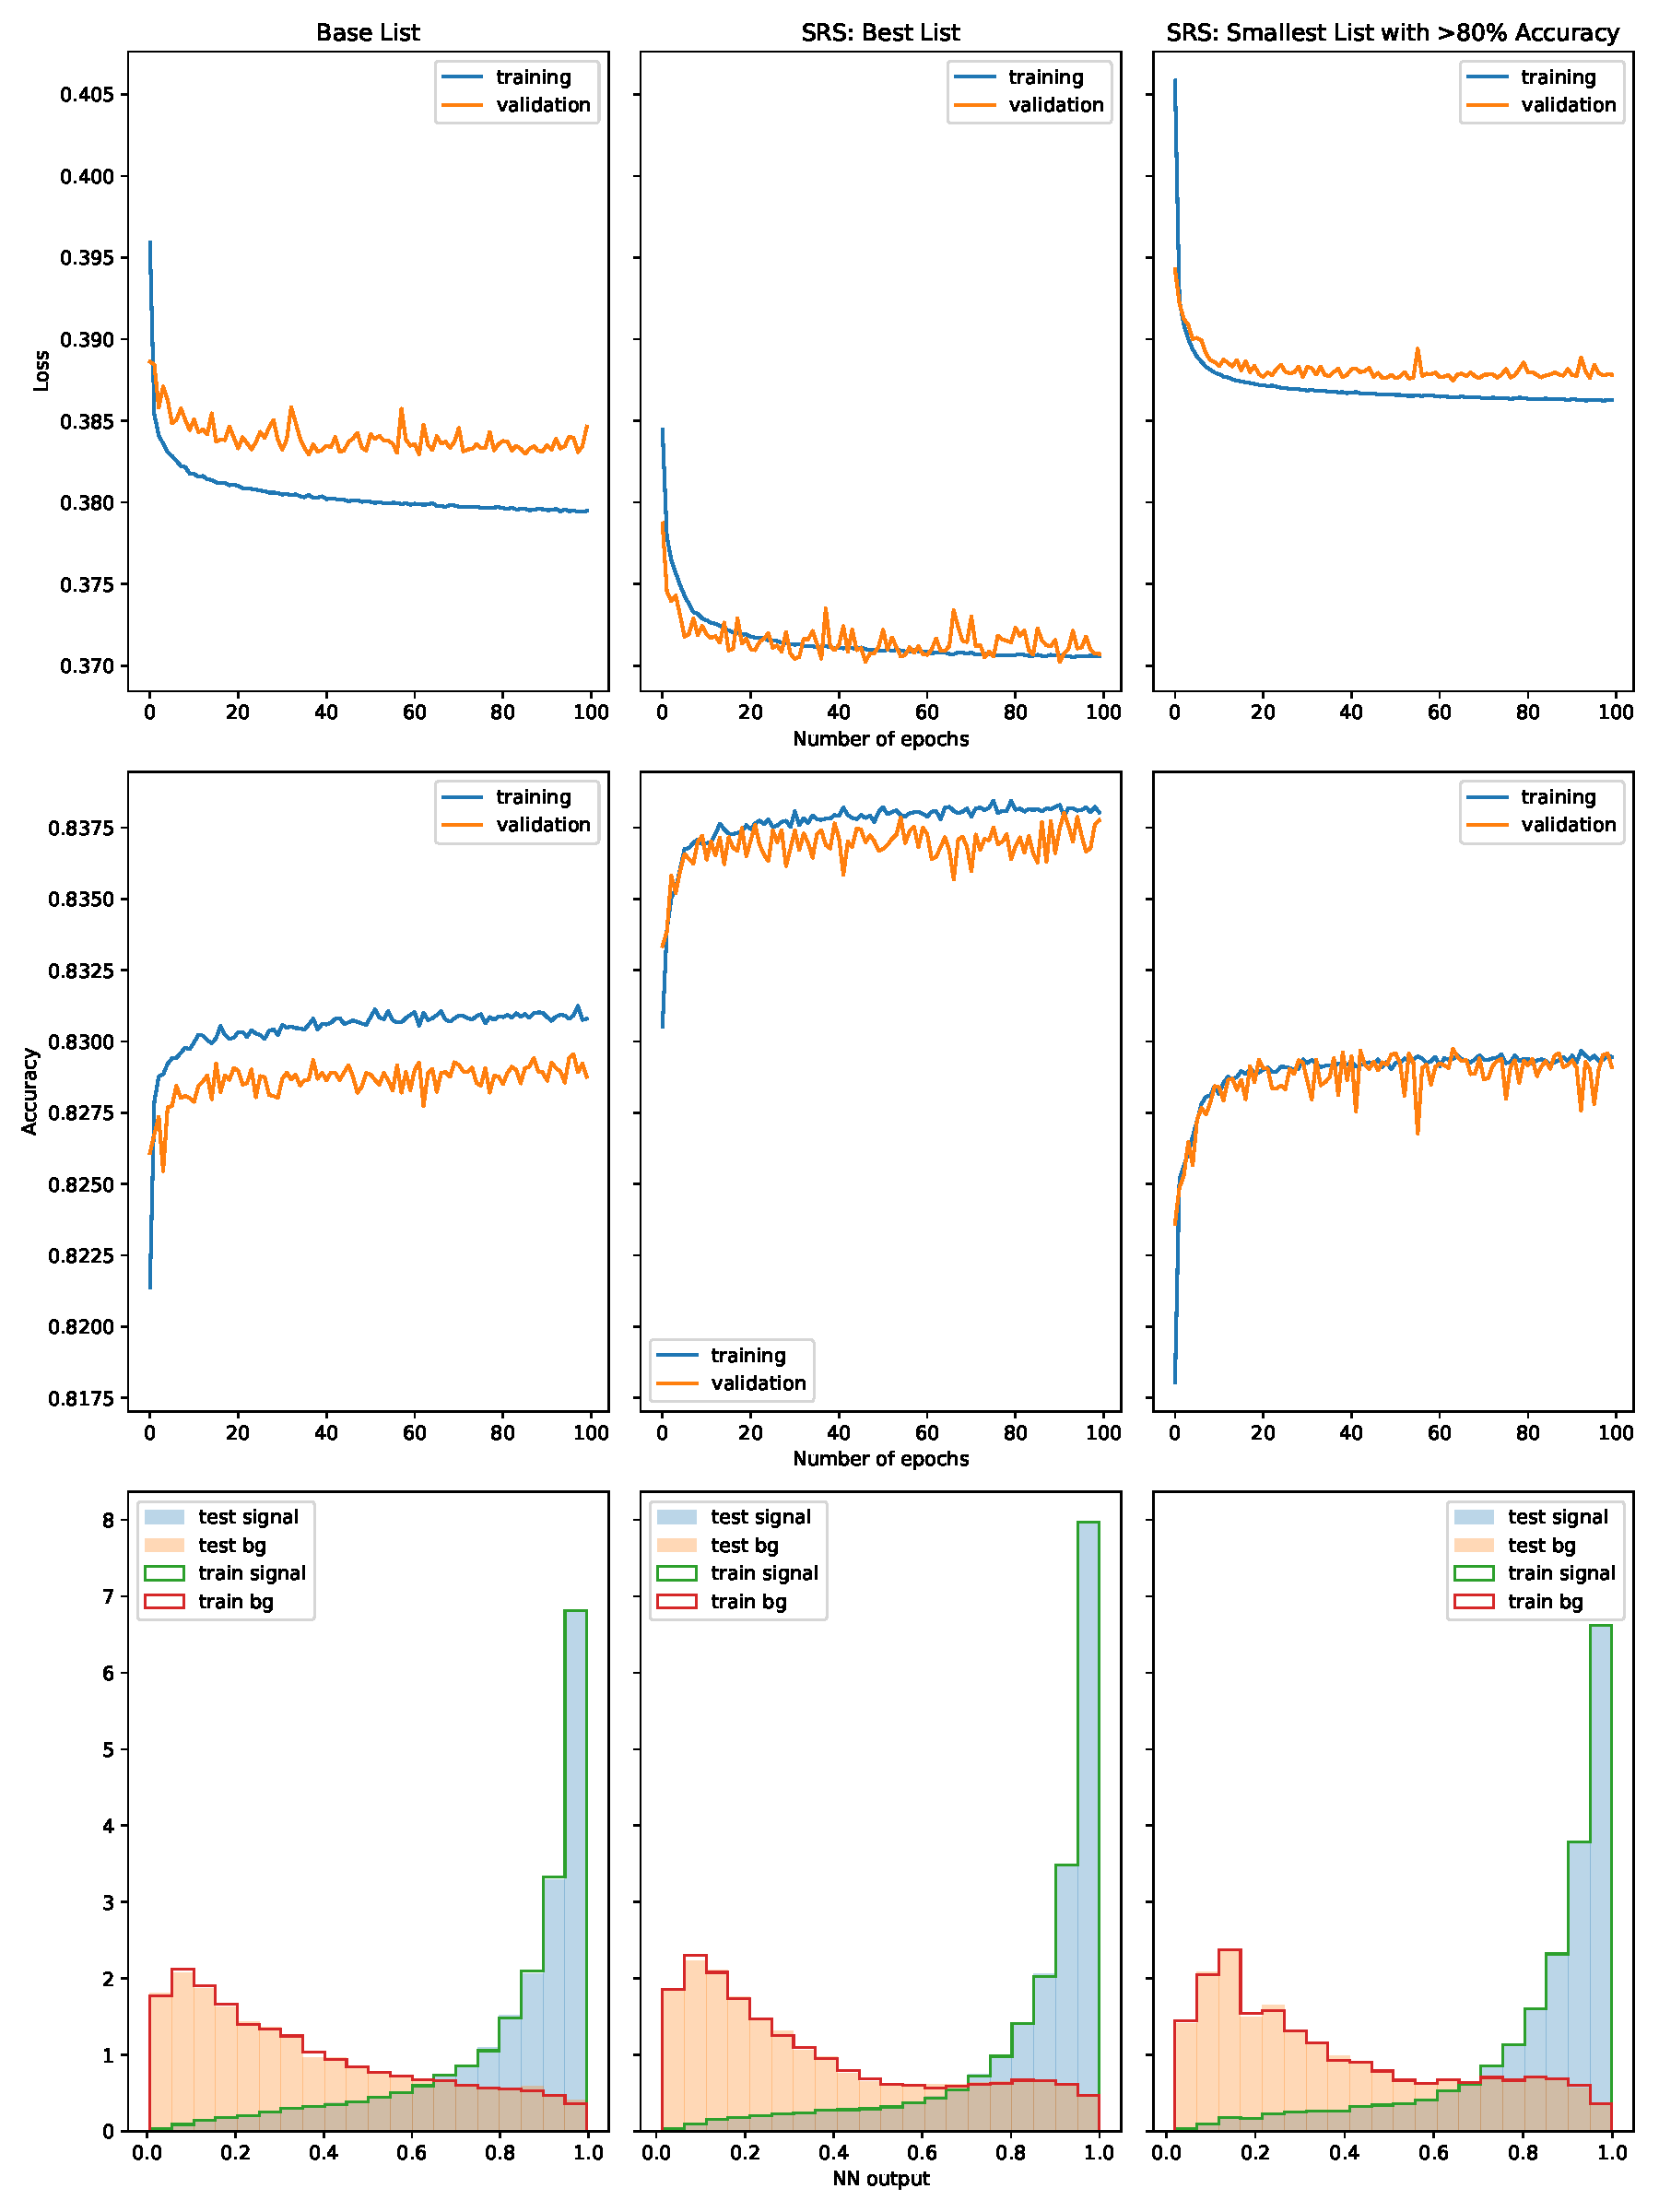
\includegraphics[width=\linewidth]{best_model/best_models.pdf}
	\caption{Performance plots of all 3 feature lists based on best parameters found for each.}
	\label{fig:best_models}
\end{figure}

\begin{figure}[ht]
	\centering
	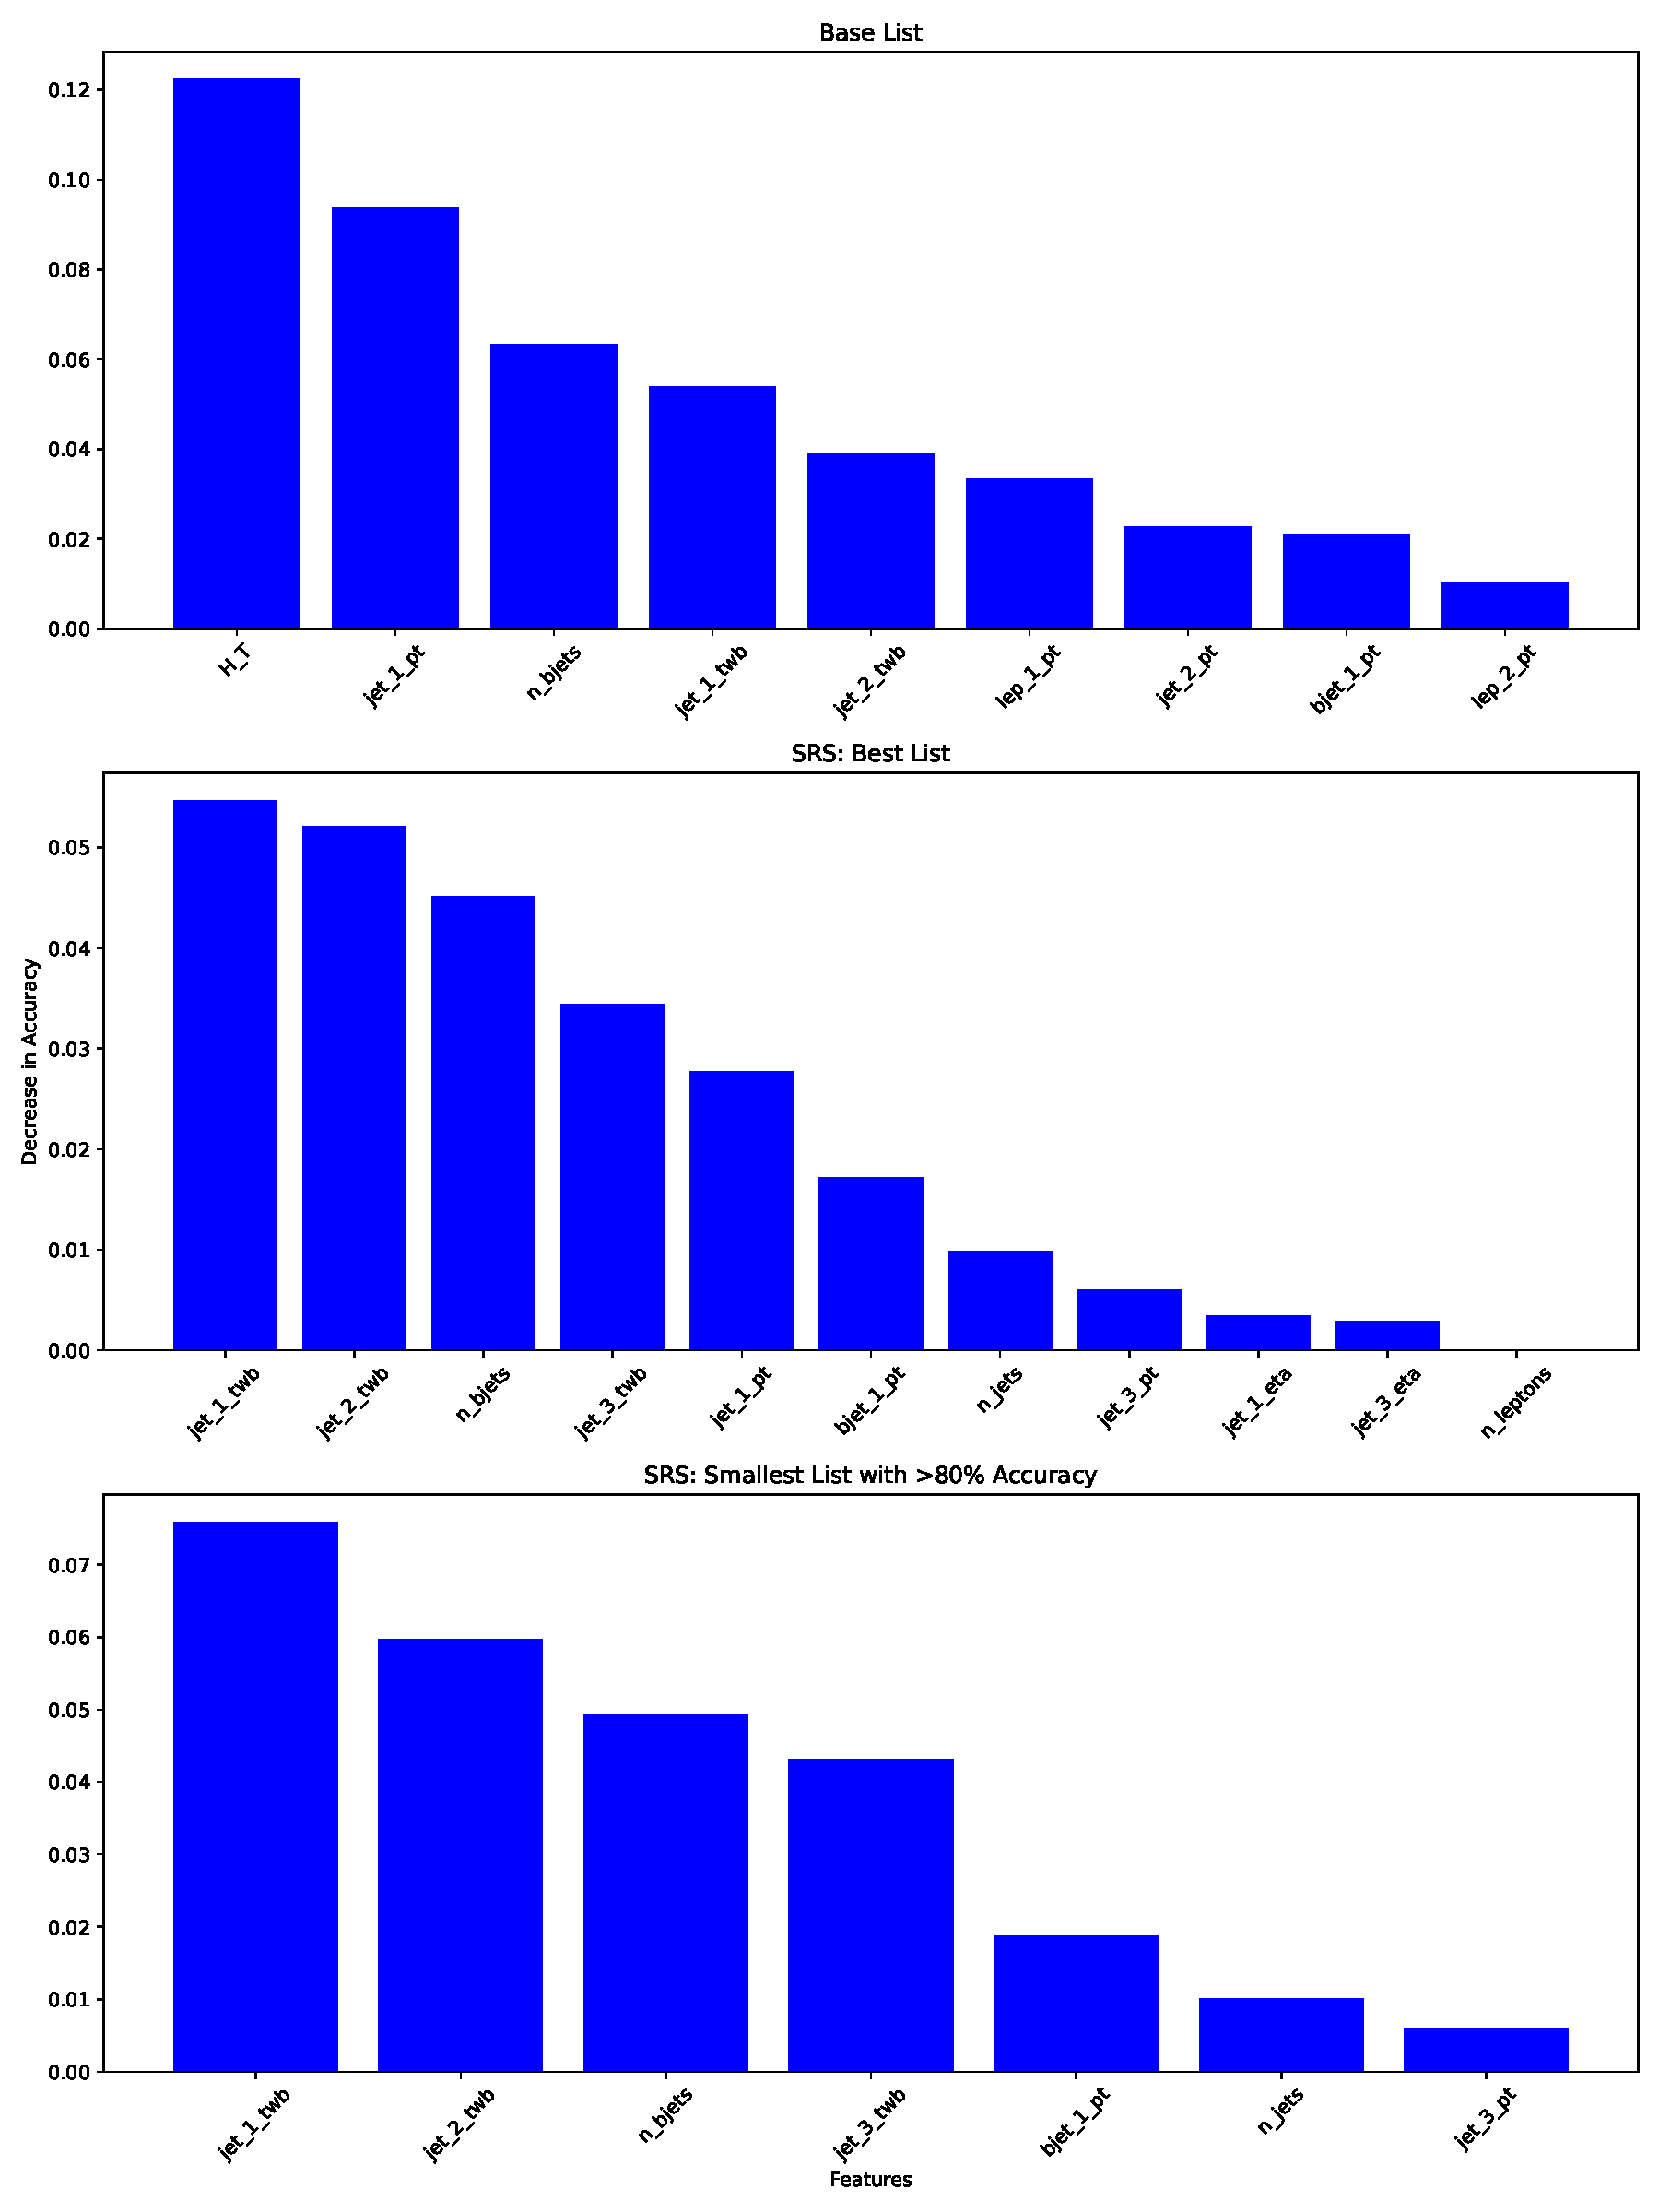
\includegraphics[width=\linewidth]{best_model/feature_importances.pdf}
	\caption{Performance plots of all 3 feature lists based on best parameters found for each.}
	\label{fig:best_models_feature_ranking}
\end{figure}



\clearpage
\section{Discussion and Summary}
– Discussion and Summary:
We were not able to improve accuracy significantly, but we we were able to show that we can reduce the dimensionality of our feature space and still maintain similiar accuracy.



Provide a concise summary of findings, successes and failures, as well as outlook for the
study.

\appendix

\clearpage
\section{Code: Base Model}

In this section we can find the code associated with the base model provided at the begining of this project. This code was used to generate the plots in Fig. \ref{fig:base_model_plots}

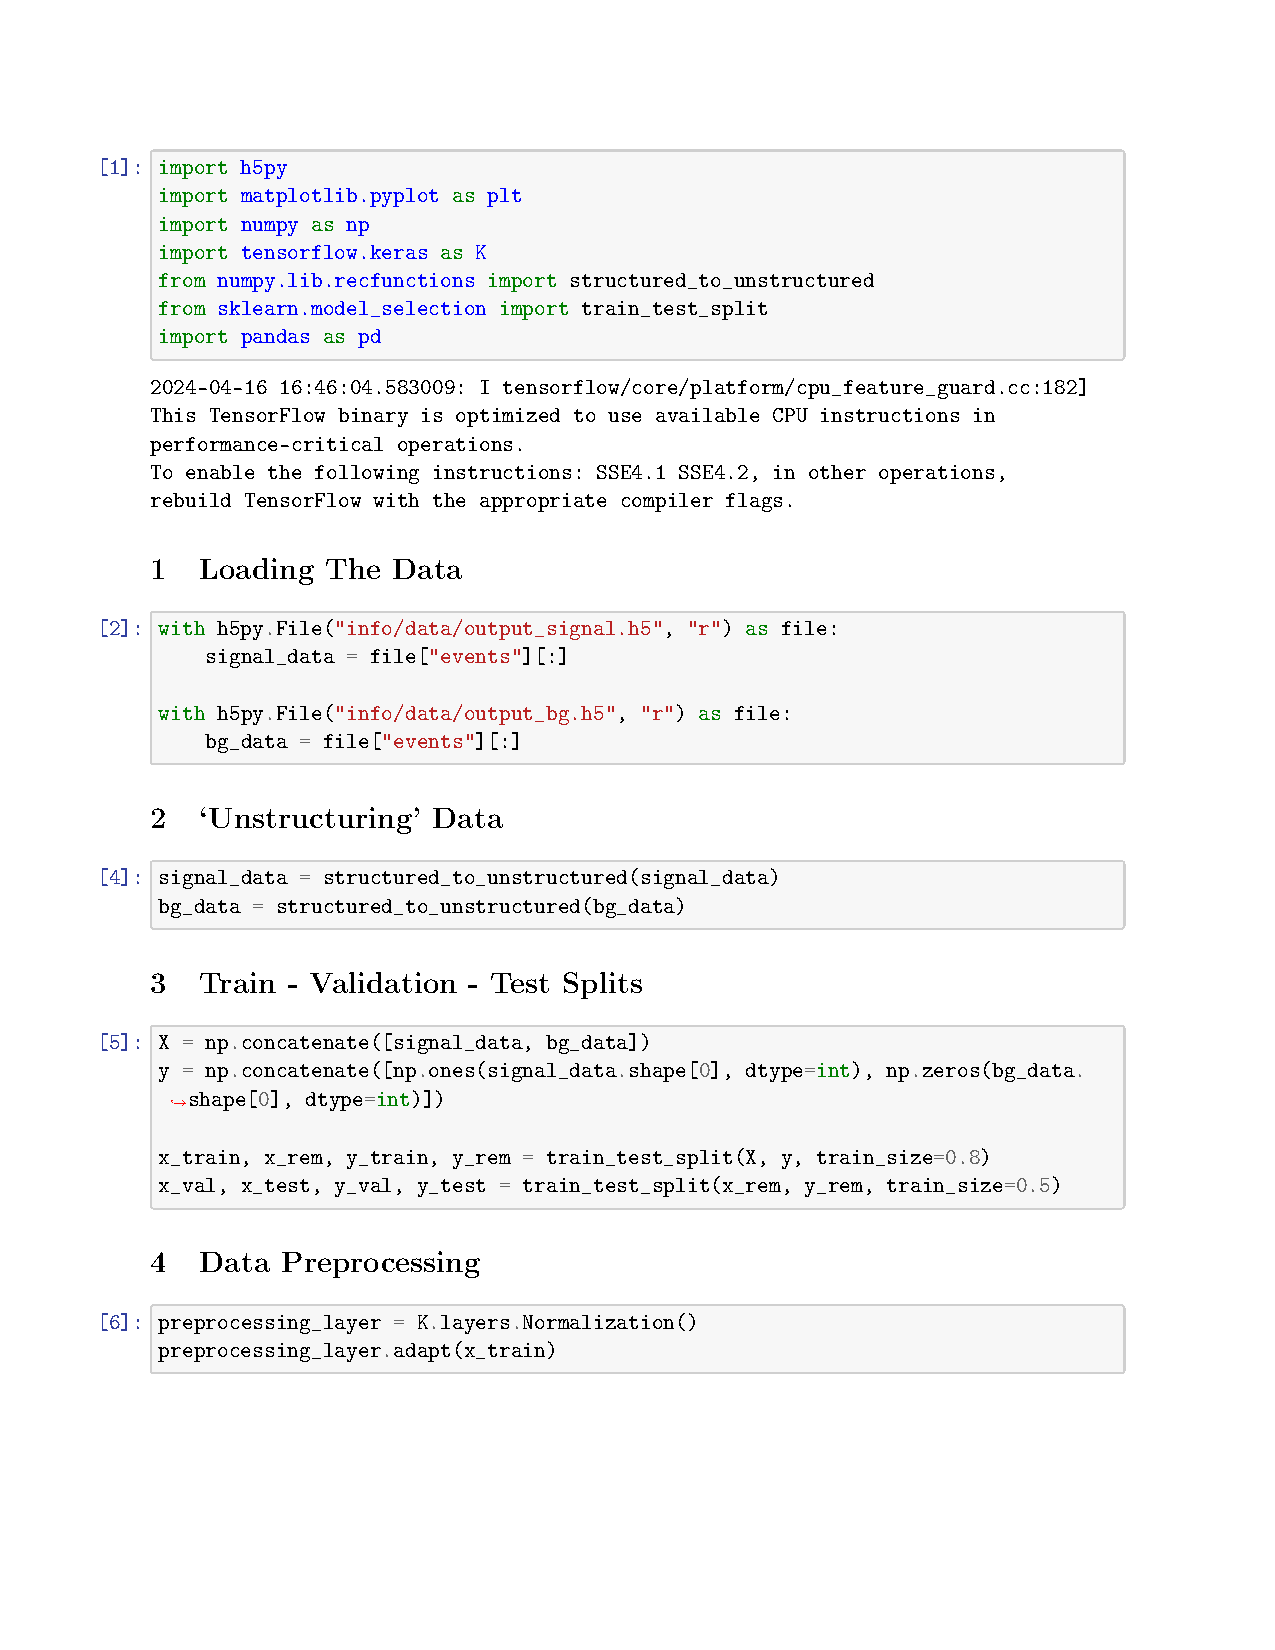
\includepdf[pages=-]{base_model/base_model.pdf}

\section{Code: Feature Selection}

In this section we can find the code associated with using the Sequential Feature Selector. This code was used to generate the plots in Fig. \ref{fig:SFS_results} and Table \ref{table:SFS_results}.

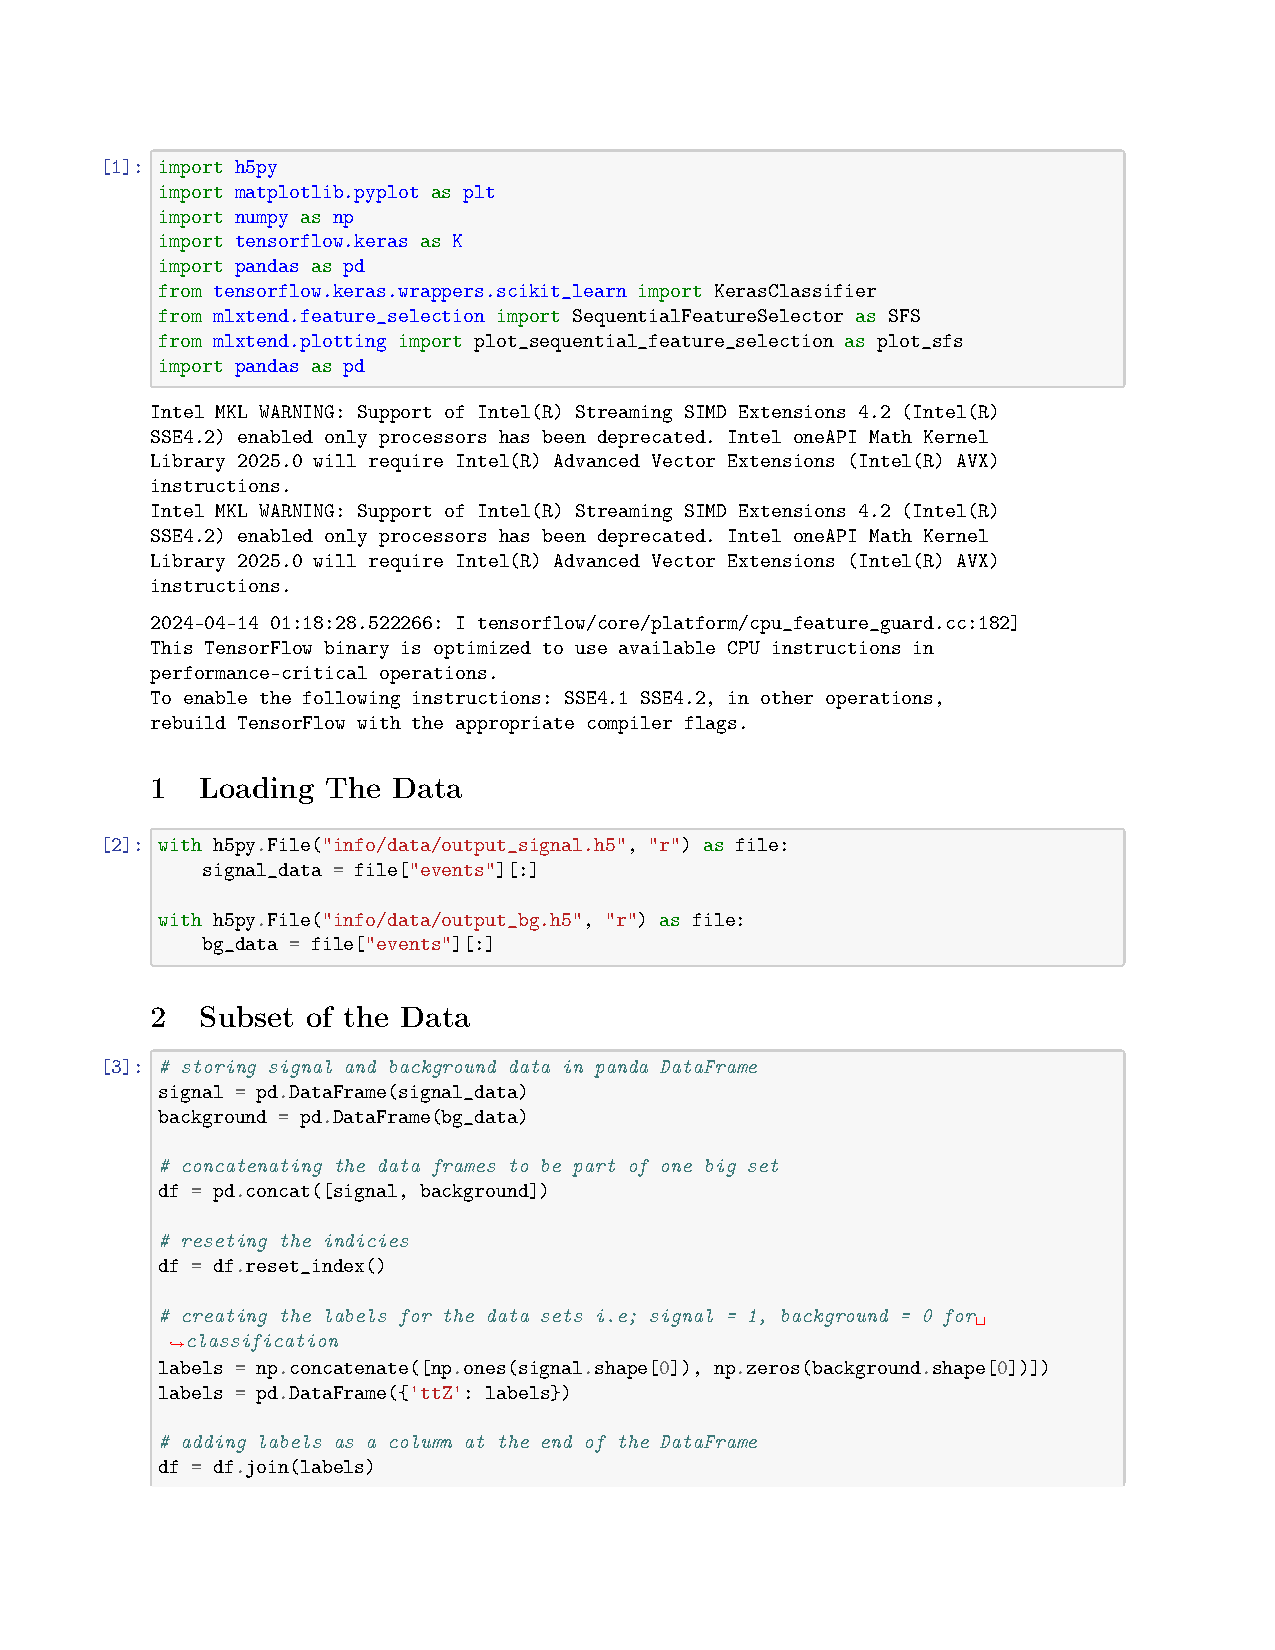
\includepdf[pages=-]{feature selection/feature_selection.pdf}

\section{Code: Feature Comparison}

This code was used to generate the plots in Fig. \ref{fig:base_models}

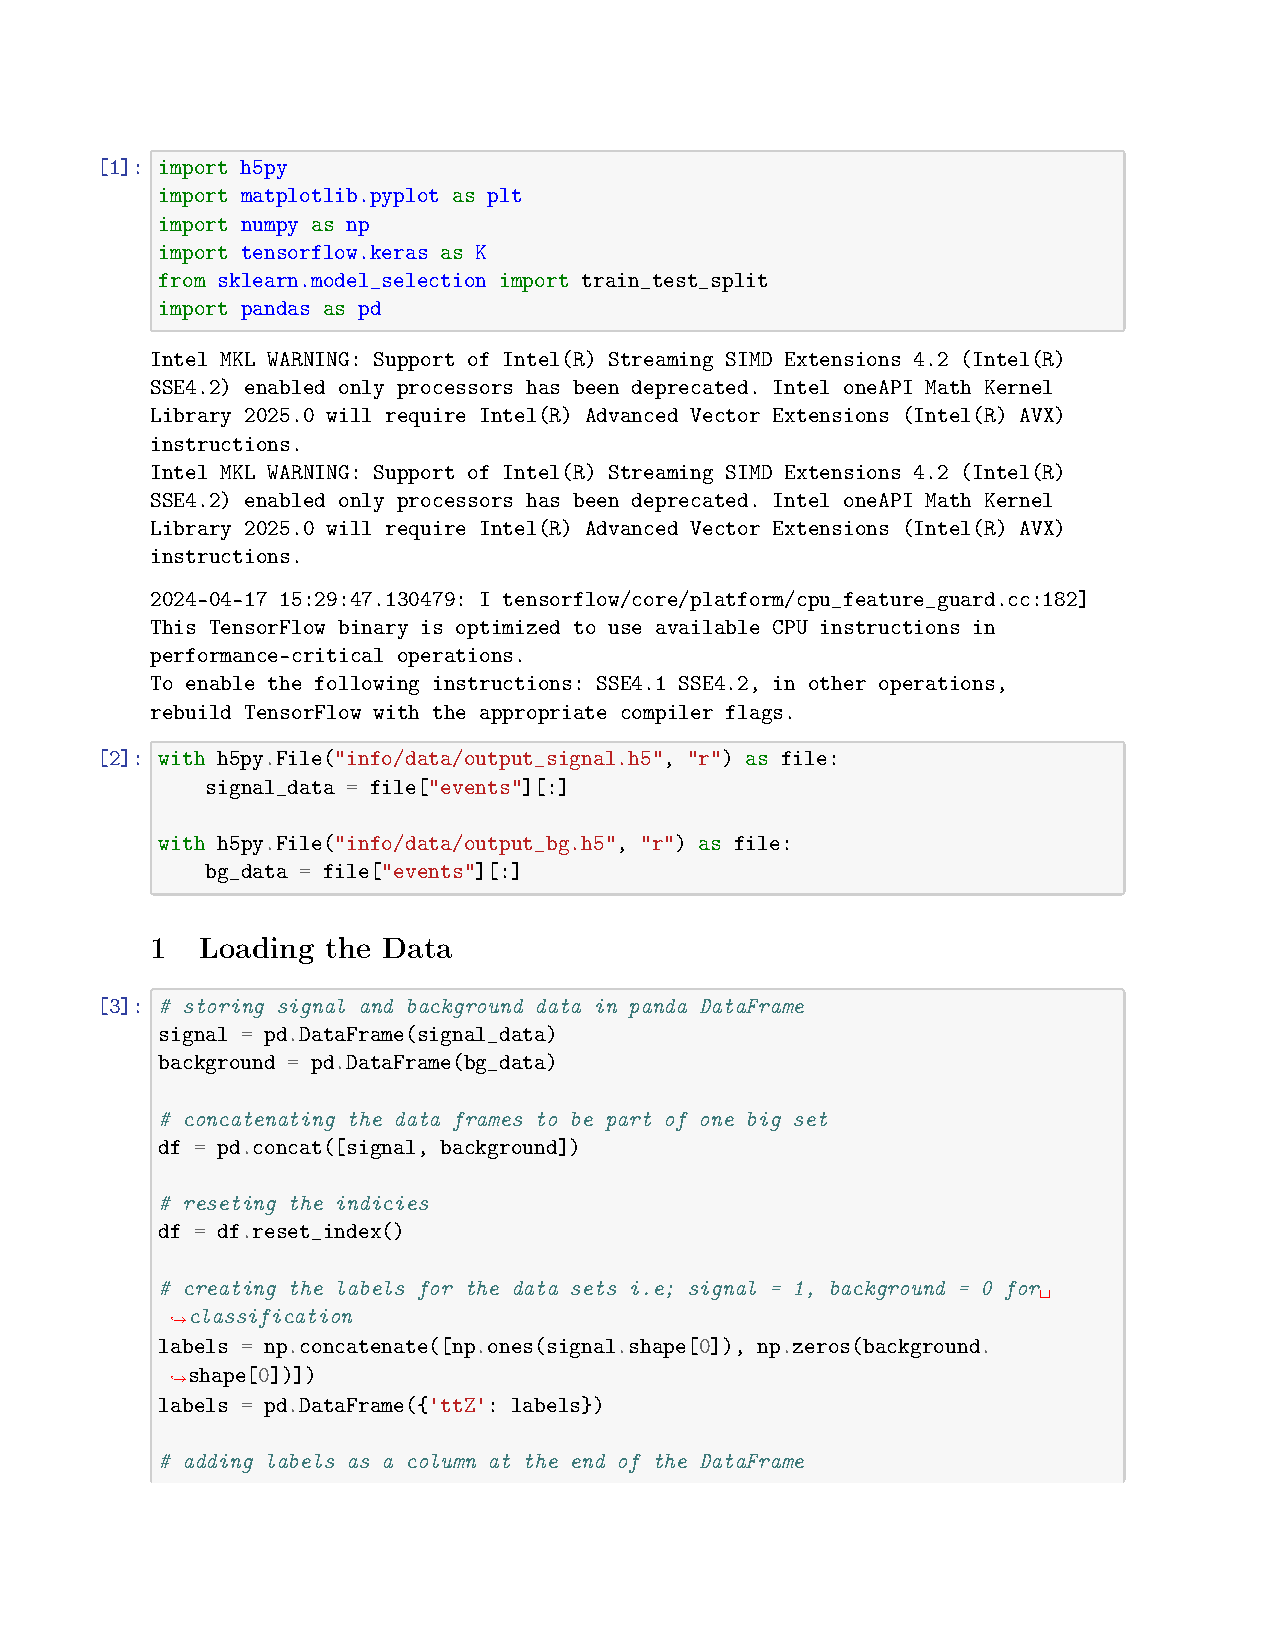
\includepdf[pages=-]{feature_comparison/feature_comparison.pdf}

\section{Code: Model Selection}

In this section we can find the code associated with using gridSearchCV for model selection. This code was used to generate the plots in Tables \ref{table:gridsearchCV_params} and \ref{table:best_params_gridsearchCV}.

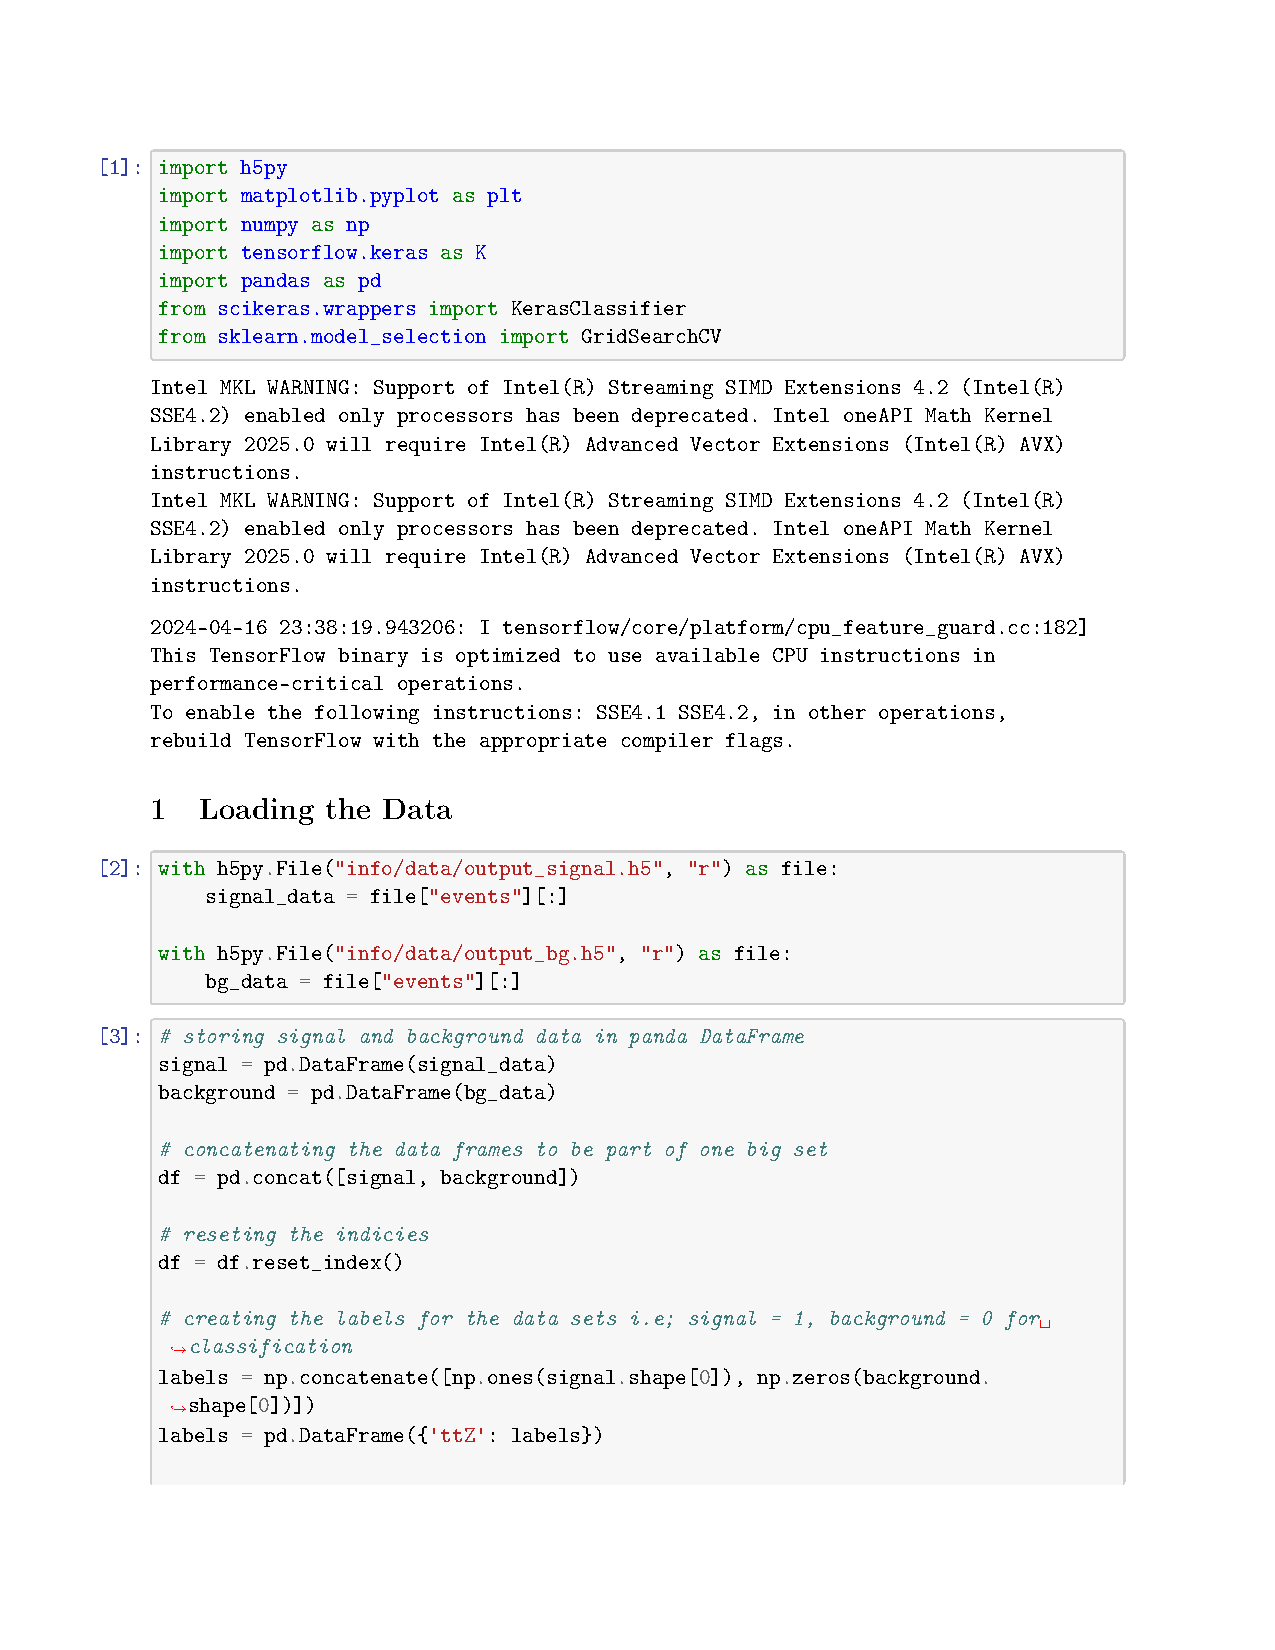
\includepdf[pages=-]{model_selection/model_selection.pdf}

\section{Code: Best Models}
This code was used to generate the plots in Fig. \ref{fig:best_models} and Fig. \ref{fig:best_models_feature_ranking}

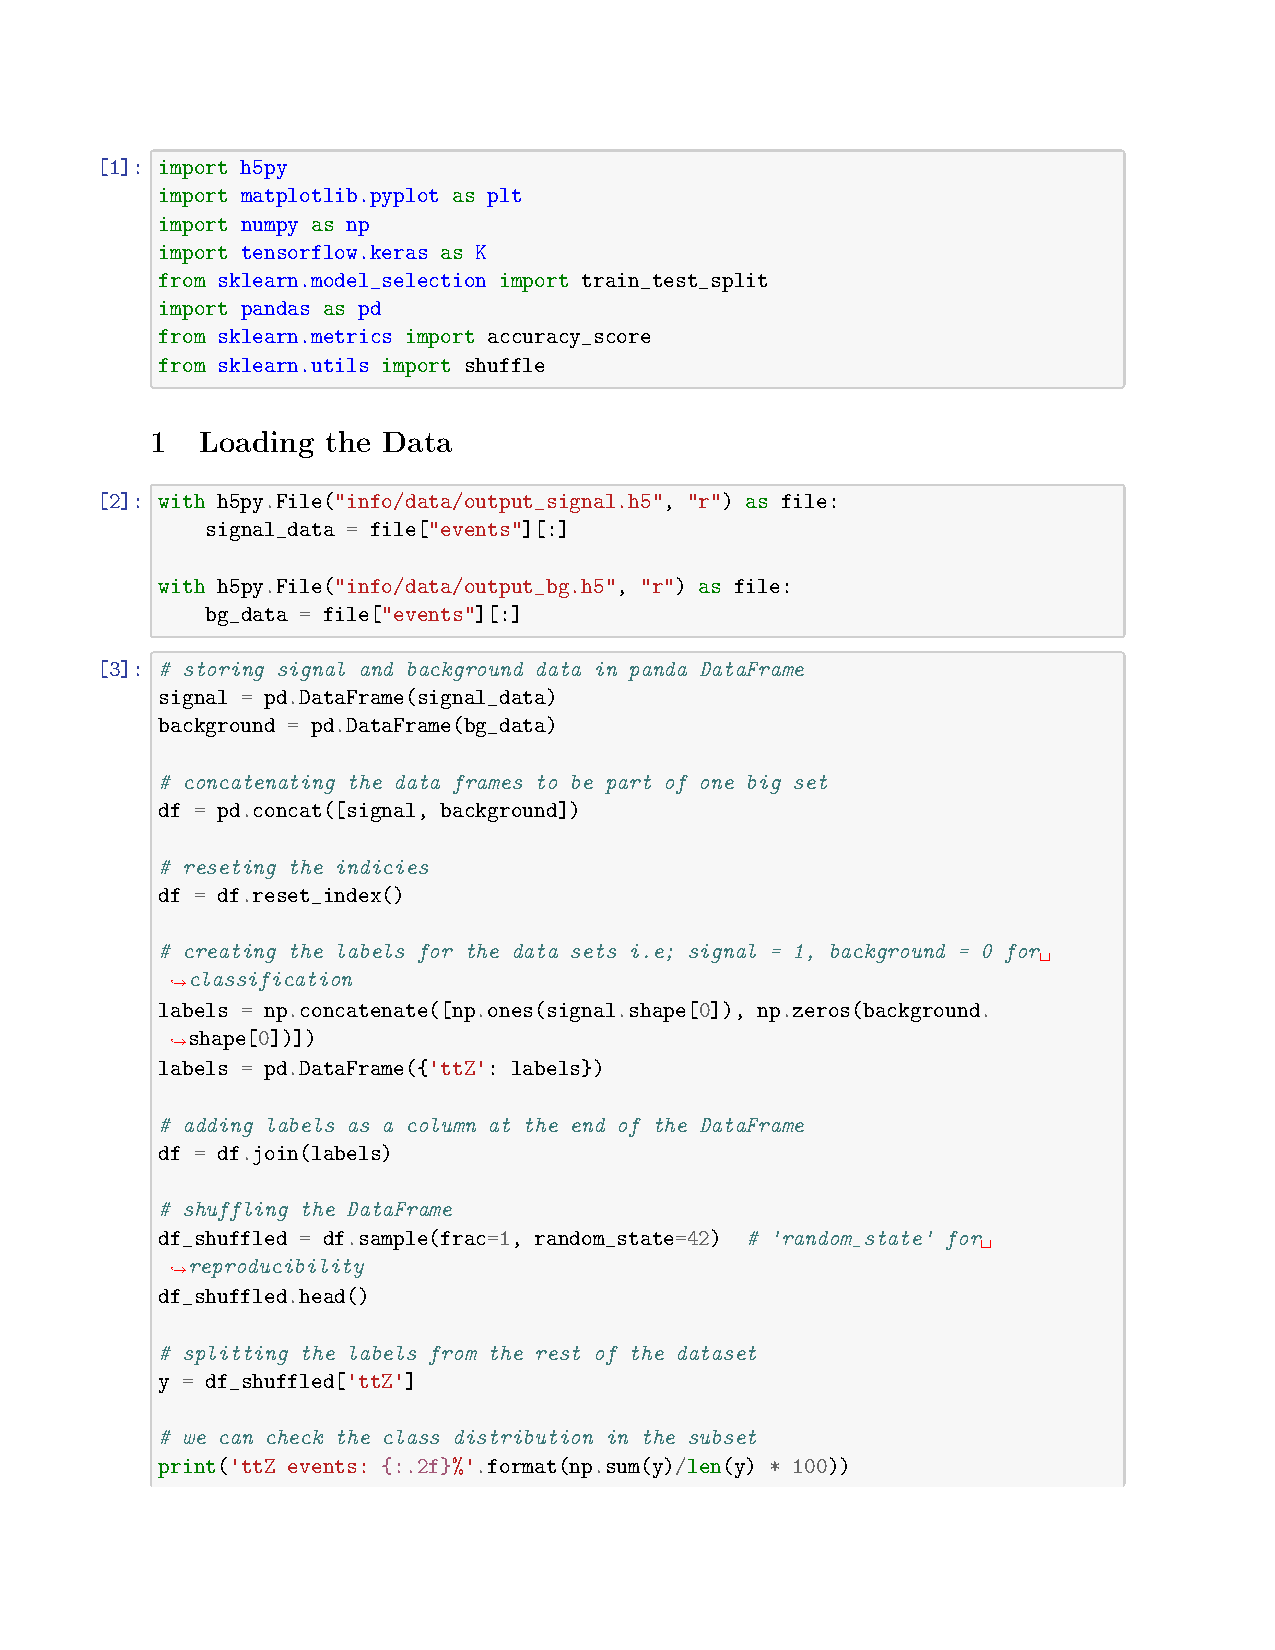
\includepdf[pages=-]{best_model/best_models_code.pdf}

\end{document}
